\documentclass[12pt,twoside]{article}
\usepackage[dvipsnames]{xcolor}
\usepackage{tikz,graphicx,amsmath,amsfonts,amscd,amssymb,bm,cite,epsfig,epsf,url,minted}
\usepackage[hang,flushmargin]{footmisc}
\usepackage[colorlinks=true,urlcolor=blue,citecolor=blue]{hyperref}
\usepackage{amsthm,multirow,wasysym,appendix}
\usepackage{array,subcaption} 
% \usepackage[small,bf]{caption}
\usepackage{bbm}
\usepackage{pgfplots}
\usetikzlibrary{spy}
\usepgfplotslibrary{external}
\usepgfplotslibrary{fillbetween}
\usetikzlibrary{arrows,automata}
\usepackage{thmtools}
\usepackage{blkarray} 
\usepackage{textcomp}
\usepackage[left=0.8in,right=1.0in,top=1.0in,bottom=1.0in]{geometry}

%% Probability operators and functions
%
% \def \P{\mathrm{P}}
\def \P{\mathrm{P}}
\def \E{\mathrm{E}}
\def \Var{\mathrm{Var}}
\let\var\Var
\def \Cov {\mathrm{Cov}} \let\cov\Cov
\def \MSE {\mathrm{MSE}} \let\mse\MSE
\def \sgn {\mathrm{sgn}}
\def \R {\mathbb{R}}
\def \C {\mathbb{C}}
\def \N {\mathbb{N}}
\def \Z {\mathbb{Z}}
\def \cV {\mathcal{V}}
\def \cS {\mathcal{S}}

\newcommand{\RR}{\ensuremath{\mathbb{R}}}

\DeclareMathOperator*{\argmin}{arg\,min}
\DeclareMathOperator*{\argmax}{arg\,max}
\newcommand{\red}[1]{\textcolor{red}{#1}}
\newcommand{\blue}[1]{\textcolor{blue}{#1}}
\newcommand{\green}[1]{\textcolor{ForestGreen}{ #1}}
\newcommand{\fuchsia}[1]{\textcolor{RoyalPurple}{ #1}}



%
%% Probability distributions
%
%\def \Bern    {\mathrm{Bern}}
%\def \Binom   {\mathrm{Binom}}
%\def \Exp     {\mathrm{Exp}}
%\def \Geom    {\mathrm{Geom}}
% \def \Norm    {\mathcal{N}}
%\def \Poisson {\mathrm{Poisson}}
%\def \Unif    {\mathrm {U}}
%
\DeclareMathOperator{\Norm}{\mathcal{N}}

\newcommand{\bdb}[1]{\textcolor{red}{#1}}

\newcommand{\ml}[1]{\mathcal{ #1 } }
\newcommand{\wh}[1]{\widehat{ #1 } }
\newcommand{\wt}[1]{\widetilde{ #1 } }
\newcommand{\conj}[1]{\overline{ #1 } }
\newcommand{\rnd}[1]{\tilde{ #1 } }
\newcommand{\rv}[1]{ \rnd{ #1}  }
\newcommand{\rM}{\rnd{ m}  }
\newcommand{\rx}{\rnd{ x}  }
\newcommand{\ry}{\rnd{ y}  }
\newcommand{\rz}{\rnd{ z}  }
\newcommand{\ra}{\rnd{ a}  }
\newcommand{\rb}{\rnd{ b}  }
\newcommand{\rt}{\rnd{ t}  }
\newcommand{\rs}{\rnd{ s}  }


\newcommand{\rpc}{\widetilde{ pc}  }
\newcommand{\rndvec}[1]{\vec{\rnd{#1}}}

\def \cnd {\, | \,}
\def \Id { I }
\def \J {\mathbf{1}\mathbf{1}^T}

\newcommand{\op}[1]{\operatorname{#1}}
\newcommand{\setdef}[2]{ := \keys{ #1 \; | \; #2 } }
\newcommand{\set}[2]{ \keys{ #1 \; | \; #2 } }
\newcommand{\sign}[1]{\op{sign}\left( #1 \right) }
\newcommand{\trace}[1]{\op{tr}\left( #1 \right) }
\newcommand{\tr}[1]{\op{tr}\left( #1 \right) }
\newcommand{\inv}[1]{\left( #1 \right)^{-1} }
\newcommand{\abs}[1]{\left| #1 \right|}
\newcommand{\sabs}[1]{| #1 |}
\newcommand{\keys}[1]{\left\{ #1 \right\}}
\newcommand{\sqbr}[1]{\left[ #1 \right]}
\newcommand{\sbrac}[1]{ ( #1 ) }
\newcommand{\brac}[1]{\left( #1 \right) }
\newcommand{\bbrac}[1]{\big( #1 \big) }
\newcommand{\Bbrac}[1]{\Big( #1 \Big)}
\newcommand{\BBbrac}[1]{\BIG( #1 \Big)}
\newcommand{\MAT}[1]{\begin{bmatrix} #1 \end{bmatrix}}
\newcommand{\sMAT}[1]{\left(\begin{smallmatrix} #1 \end{smallmatrix}\right)}
\newcommand{\sMATn}[1]{\begin{smallmatrix} #1 \end{smallmatrix}}
\newcommand{\PROD}[2]{\left \langle #1, #2\right \rangle}
\newcommand{\PRODs}[2]{\langle #1, #2 \rangle}
\newcommand{\der}[2]{\frac{\text{d}#2}{\text{d}#1}}
\newcommand{\pder}[2]{\frac{\partial#2}{\partial#1}}
\newcommand{\derTwo}[2]{\frac{\text{d}^2#2}{\text{d}#1^2}}
\newcommand{\ceil}[1]{\lceil #1 \rceil}
\newcommand{\Imag}[1]{\op{Im}\brac{ #1 }}
\newcommand{\Real}[1]{\op{Re}\brac{ #1 }}
\newcommand{\norm}[1]{\left|\left| #1 \right|\right| }
\newcommand{\norms}[1]{ \| #1 \|  }
\newcommand{\normProd}[1]{\left|\left| #1 \right|\right| _{\PROD{\cdot}{\cdot}} }
\newcommand{\normTwo}[1]{\left|\left| #1 \right|\right| _{2} }
\newcommand{\normTwos}[1]{ \| #1  \| _{2} }
\newcommand{\normZero}[1]{\left|\left| #1 \right|\right| _{0} }
\newcommand{\normTV}[1]{\left|\left| #1 \right|\right|  _{ \op{TV}  } }% _{\op{c} \ell_1} }
\newcommand{\normOne}[1]{\left|\left| #1 \right|\right| _{1} }
\newcommand{\normOnes}[1]{\| #1 \| _{1} }
\newcommand{\normOneTwo}[1]{\left|\left| #1 \right|\right| _{1,2} }
\newcommand{\normF}[1]{\left|\left| #1 \right|\right| _{\op{F}} }
\newcommand{\normLTwo}[1]{\left|\left| #1 \right|\right| _{\ml{L}_2} }
\newcommand{\normNuc}[1]{\left|\left| #1 \right|\right| _{\ast} }
\newcommand{\normOp}[1]{\left|\left| #1 \right|\right|  }
\newcommand{\normInf}[1]{\left|\left| #1 \right|\right| _{\infty}  }
\newcommand{\proj}[1]{\mathcal{P}_{#1} \, }
\newcommand{\diff}[1]{ \, \text{d}#1 }
\newcommand{\vc}[1]{\boldsymbol{\vec{#1}}}
\newcommand{\rc}[1]{\boldsymbol{#1}}
\newcommand{\vx}{\vec{x}}
\newcommand{\vy}{\vec{y}}
\newcommand{\vz}{\vec{z}}
\newcommand{\vu}{\vec{u}}
\newcommand{\vv}{\vec{v}}
\newcommand{\vb}{\vec{\beta}}
\newcommand{\va}{\vec{\alpha}}
\newcommand{\vaa}{\vec{a}}
\newcommand{\vbb}{\vec{b}}
\newcommand{\vg}{\vec{g}}
\newcommand{\vw}{\vec{w}}
\newcommand{\vh}{\vec{h}}
\newcommand{\vbeta}{\vec{\beta}}
\newcommand{\valpha}{\vec{\alpha}}
\newcommand{\vgamma}{\vec{\gamma}}
\newcommand{\veta}{\vec{\eta}}
\newcommand{\vnu}{\vec{\nu}}
\newcommand{\rw}{\rnd{w}}
\newcommand{\rvnu}{\vc{\nu}}
\newcommand{\rvv}{\rndvec{v}}
\newcommand{\rvw}{\rndvec{w}}
\newcommand{\rvx}{\rndvec{x}}
\newcommand{\rvy}{\rndvec{y}}
\newcommand{\rvz}{\rndvec{z}}
\newcommand{\rvX}{\rndvec{X}}


\newtheorem{theorem}{Theorem}[section]
% \declaretheorem[style=plain,qed=$\square$]{theorem}
\newtheorem{corollary}[theorem]{Corollary}
\newtheorem{definition}[theorem]{Definition}
\newtheorem{lemma}[theorem]{Lemma}
\newtheorem{remark}[theorem]{Remark}
\newtheorem{algorithm}[theorem]{Algorithm}

% \theoremstyle{definition}
%\newtheorem{example}[proof]{Example}
\declaretheorem[style=definition,qed=$\triangle$,sibling=definition]{example}
\declaretheorem[style=definition,qed=$\bigcirc$,sibling=definition]{application}

%
%% Typographic tweaks and miscellaneous
%\newcommand{\sfrac}[2]{\mbox{\small$\displaystyle\frac{#1}{#2}$}}
%\newcommand{\suchthat}{\kern0.1em{:}\kern0.3em}
%\newcommand{\qqquad}{\kern3em}
%\newcommand{\cond}{\,|\,}
%\def\Matlab{\textsc{Matlab}}
%\newcommand{\displayskip}[1]{\abovedisplayskip #1\belowdisplayskip #1}
%\newcommand{\term}[1]{\emph{#1}}
%\renewcommand{\implies}{\;\Rightarrow\;}



\begin{document}

\begin{center}
{\large{\textbf{Homework 1}} } \vspace{0.2cm}\\
Due Jan 29 at 11 pm
\\
\end{center}
Unless stated otherwise, justify any answers you give.
You can work in groups, but each
student must write their own solution based on their own
understanding of the problem.

When uploading your homework to Gradescope you will have to
select the relevant pages for each question.  Please submit each
problem on a separate page (i.e., 1a and~1b can be on the same page but 1
and 2 must be on different pages).  We understand that this may be
cumbersome but this is the best way for the grading team to grade your
homework assignments and provide feedback in a timely manner.  Failure
to adhere to these guidelines may result in a loss of points.
Note that it may take some time to
select the pages for your submission.  Please plan accordingly.  We
suggest uploading your assignment at least 30 minutes before the deadline
so you will have ample time to select the correct pages for your
submission.  If you are using \LaTeX, consider using the minted or
listings packages for typesetting code.  
\\

\begin{enumerate}

\item (Three random variables) If a random variable $\rnd{w}$ is positively correlated with another random variable $\rnd{y}$, and $\rnd{y}$ is positively correlated with a third random variable $\rnd{z}$, can $\rnd{w}$ and $\rnd{z}$ be negatively correlated? Provide an example, or prove that it is impossible.
\begin{itemize}
    \item this is false, as a counter example consider a Gaussian random vector $\begin{pmatrix} \rnd{y}\\ \rnd{w}\\ \rnd{z}\end{pmatrix}$ with $\mu_{w}=\mu_{y}=\mu_{z}=0$ and covariance matrix $\Sigma=\begin{pmatrix}
        1&.5&.5\\
        .5 & 1 & -.25\\
        .5 & -.25 &1
    \end{pmatrix}$
    \item we can verify that $\Sigma$ has all positive eigenvalues and thus is positive semi definite full rank, invariable and thus a valid Gaussian random vector 
    \item  so now we can compute the covariance between each variable 
    \item $cov(w,y)=E[w,y]+E[w]E[y]$ further since we set both these variables to have zero mean we have $cov(w,y)=E[w,y]=\rho_{w,y}=.5$ using the result from textbook example 8.8 or recitation 1 question 2. 
    \item we can do the same for $cov(y,z)=E[y*z]-E[y]E[y]=.5$
    \item by the same logic however we can see that $cov(w,z)=E[w*z]-E[w]E[z]=-.25$ 
    \item thus y is positively correlated with both w and z, but w and z are negatively correlated with one another so we have a counter example. 
\end{itemize}

\item (Averaging noisy data) We want to estimate a signal represented by a zero-mean random variable $\rx$ with unit variance. We have access to $n$ measurements $\ry_1$, $\ry_2$, \ldots, $\ry_n$, where $\ry_i := \rx + \rz_i$ for $1\leq i \leq n$. Each $\rz_i$ is a zero-mean random variable with variance $\sigma^2$. The random variables $\rx$, $\rz_1$, $\rz_2$, \ldots, $\rz_n$ are all mutually independent. We decide to estimate $\rx$ by scaling the sum of all measurements: the estimator is $\alpha \sum_{i=1}^{n}\ry_i$ for some $\alpha \in \R$.
\begin{enumerate} 
\item What value of $\alpha$ minimizes the mean squared error? 


\begin{itemize}
    \item mean squared error can be expressed as a function of $\alpha$ as $mse(\alpha)=E[(x-\alpha\Sigma_{i=1}^{n}y_i)^2]$
    \item this can be expanded as $mse(\alpha)=E[(x-\alpha\Sigma_{i=1}^{n}y_i)^2]=E[x^2-2\alpha x\Sigma_{i=1}^{n}y_i+\alpha^2\Sigma_{i=1}^{n}y_i^2]=E[x^2]-2\alpha E[x\Sigma_{i=1}^{n}y_i]+\alpha^2E[\Sigma_{i=1}^{n}y_i^2]$
    \item we know that $\Tilde{x}$ has mean 0 and variance 1 that is  $var(x)=E[x^2]-E[x]^2=E[x^2]=1$ meaning we can write $mse(\alpha)=E[(x-\alpha\Sigma_{i=1}^{n}y_i)^2]=1-2\alpha E[x\Sigma_{i=1}^{n}y_i]+\alpha^2E[\Sigma_{i=1}^{n}y_i^2]$
    \item now we can use the definition of $y_i=x+z_{i}$ to write $mse(\alpha)=1-2\alpha E[x\Sigma_{i=1}^{n}(x+z_{i})]+\alpha^2E[\Sigma_{i=1}^{n}(x+z_{i})^2]=1-2n\alpha E[x^2]-2\alpha E[x\Sigma_{i=1}^{n}(z_{i})]+\alpha^2E[\Sigma_{i=1}^{n}(x^2+2xz_{i}+z_{i}^2)]=1-2n\alpha E[x^2]-2\alpha E[x\Sigma_{i=1}^{n}(z_{i})]+\alpha^2nE[(x^2)]+\alpha^2E[\Sigma_{i=1}^{n}2xz_{i}]+\alpha^2E[\Sigma_{i=1}^{n}(z_{i}^2)]=1-2n\alpha-2\alpha E[x]\Sigma_{i=1}^{n}E[z_i]+\alpha^2n+2\alpha^2E[x]\Sigma_{i=1}^{n}E[z_i]+\alpha^2\Sigma_{i=1}^{n}E[z_i^2]=1-2n\alpha-2\alpha E[x]\Sigma_{i=1}^{n}E[z_i]+\alpha^2n+2\alpha^2E[x]\Sigma_{i=1}^{n}E[z_i]+\alpha^2n\sigma^2$
    \item then we recall that $E[z_i]=E[x]=0$ meaning $mse(\alpha)=1-2n\alpha+\alpha^2n+\alpha^2n\sigma^2$
    \item now we can take the first derivative of that expression with respect to $\alpha$ and see that $MSE(\alpha)'=-2n+2\alpha n +2\alpha n\sigma^2$
    \item we can further see that $MSE(\alpha)''=2n+2n\sigma^2$ since n is the number of data points and thus must greater than zero and $\sigma^2$ is a variance and thus must be greater than zero we know that the function is convex and thus any point where the first derivative is zero will be a global minima 
    \item thus we can set $MSE(\alpha)'=-2n+2\alpha n +2\alpha n\sigma^2=0$ and get $\alpha=\frac{1}{1+\sigma^2}$
    \item \textbf{Look in pictures, i hand wrote a potentially nicer derivation that reaches the same conclusion, might be good to update}
\end{itemize}
\item What does the estimator tend to when $\sigma^2 \rightarrow 0$ and $\sigma^2 \rightarrow \infty$? 

\begin{itemize}
    \item i found that the optimal $\alpha$ was $\alpha_{mmse}=\frac{1}{1+\sigma^2}$
    \item so as as $\sigma^2$ goes to 0 $\alpha_{mmse}$ goes to 1
    \item as $\sigma^2$ goes to infinity $\alpha_{mmse}$ goes to zero
\end{itemize}
\item What is the mean squared error of the estimator? How does it scale with $n$?
\begin{itemize}
\item we can write mean squared error ended as $mse(\alpha)=1-2n\alpha+\alpha^2n+\alpha^2n\sigma^2$
\item evaluating this expression at our estimator $\alpha_{ols}$yields  $mse(\alpha_{ols})=1-2n\alpha_{ols}+\alpha_{ols}^2n+\alpha_{ols}^2n\sigma^2=1-\frac{2n}{1+\sigma^2}+\frac{n}{(1+\sigma^2)^2}+\frac{n\sigma^2}{(1+\sigma^2)^2}=1+n(\frac{1}{(1+\sigma^2)^2}+\frac{\sigma^2}{(1+\sigma^2)^2}-\frac{2}{1+\sigma^2})=1+n(\frac{1+\sigma^2}{(1+\sigma^2)^2}-\frac{2}{1+\sigma^2})=1+n(\frac{1+\sigma^2}{(1+\sigma^2)(1+\sigma^2)}-\frac{2}{1+\sigma^2})=1+n(\frac{1}{(1+\sigma^2)}-\frac{2}{1+\sigma^2})=1-\frac{n}{1+\sigma^2}$
\item thus we can see that the mean squared error of our estimator is decreasing in the number of observations n
\end{itemize}
\end{enumerate}

\item (Interference) We model a signal of interest as a random variable $\ra$ with mean $\mu$ and variance $\sigma^2$, which is known to be nonnegative. The signal cannot be observed directly. The available measurement is modeled as a random variable $\ry$ which equals $\rnd{w}\ra$, where $\rnd{w}$ is an interfering signal that is equal to -1 with probability 1/2 and 1 with probability 1/2. We assume that  $\rnd{w}$ and $\ra$ are independent.
\begin{enumerate} 
\item What is the linear MMSE estimator of $\ra$ given $\ry=y$? 

\begin{itemize}
    \item from lecture we know that the linear MMSE estimator of a given y will be given by $l(y)=\sigma\rho_{y,a}\frac{y-\mu_{y}}{\sigma_{y}}+\mu$
    
    
    \item so first we want to compute $\mu_{y}$ we know that $y=wa$ and assume that a and y are independent thus $E[y]=E[wa]=E[w]E[a]$ 
    \item $E[w]=\frac{1}{2}(-1)+\frac{1}{2}(1)=0$  thus we have $E[y]=E[wa]=E[w]E[a]=\mu0=0$
    \item now we want to find the variance of y $var(y)=var(wa)=E[(wa)^2]-E[wa]^2=E[w^2a^2]-E[wa]$ we can show that given $w,a$ are independent then $w^2,a^2$ are independent as $P(w)=P(w|a)$ meaning $P(w)=P(w|a^2)$ and further that  $P(x^2)=P(x^2|y^2)$ so we can assert  $var(y)=var(wa)=E[w^2]E[a^2]-E[w]E[a]$ and as $E[w]=0$ we have $var(y)=var(wa)=E[w^2]E[a^2]$ 
    \item we can solve $E[w^2]=\frac{1}{2}1^2+\frac{1}{2}(-1)^2=1$ and as we know $var(a)=E[a^2]-E[a]^2=\sigma^2$can express $E[a^2]=\mu^2+\sigma^2$ and thus we see $var(y)=var(wa)=E[w^2]E[a^2]=1(\mu^2+\sigma^2)=\sigma^2+\mu^2$
    \item now we need to calculate the coefficient of correlation between a,y. so first we see $Cov(a,y)=E[ay]-E[a]E[y]=E[a(wa)]-E[a]E[wa]=E[wa^2]-E[a]E[w]E[a]=E[wa^2]-E[w]E[a]^2$
    \begin{itemize}
        \item we can take a second to show that$w,a^2$ are independent 
        \item first note that we know a is non negative and that w and a are independent
        \item so we can write $P(a^2\leq a, w\leq w)=P(-\sqrt{a}\leq a \leq \sqrt{a}, w\leq w)=P(a\leq \sqrt{a}, w\leq w)-P(a\leq -\sqrt{a}, w\leq w)=P(w\leq w)P(a\leq \sqrt{a})-P(a\leq -\sqrt{a})P(w\leq w)=P(w\leq w)(P(a\leq \sqrt{a})-P(a\leq -\sqrt{a}))=(a^2\leq a)P(w\leq w)$ showing the result
    \end{itemize}
    \item so this allows us to write $Cov(a,y)=E[wa^2]-E[w]E[a]^2=E[w]E[a^2]-E[w]E[a]^2$
    \item as we showed above $E[a^2]=\sigma^2+\mu^2$ and $E[w]=0$ and $E[a]=\mu$ 
    \item so finally we get$Cov(a,y)=E[wa^2]-E[w]E[a]^2=E[w]E[a^2]-E[w]E[a]^2=0(\mu^2+\sigma^2)-0\mu^2=0$
    \item so this tells us that  $\rho_{a,b}=0$ meaning a and y are uncorrelated
    \item so finally we have $l(y)=\sigma\rho_{y,a}\frac{y-\mu_{y}}{\sigma_{y}}+\mu=0+\mu=\mu$
\end{itemize}
\item What is the MSE of the linear MMSE estimator? 
\begin{itemize}
    \item the mean squared error of our estimator $\ell$is $mse(\ell)=E[(\ell -a)^2]=E[(\mu-a)^2]=E[a^2-2\mu a -\mu^2]=E[a^2]-2\mu E[a]+\mu^2=\sigma^2+\mu^2-2\mu^2+\mu^2=\sigma^2$ this makes sense as we are just choosing the mean and the variance is effectively defined as the mean squared error of this choice. 
\end{itemize}


\item Propose a nonlinear estimator that has a better MSE than the linear MMSE.

\begin{itemize}
    \item we could chose the conditional mean function ie $\mu_{a|y}(y)=\Sigma_{a\in A}af_{a|y}(a|y)$ as discussed in lecture this would do better at finding subgroups in our population which would presumably be based on if the resistance we positive or negative.
\end{itemize}

\end{enumerate}

\item (Temperature) The table in \texttt{tempature.csv} includes the average temperatures of each month at different locations (longitude and latitude). 

\begin{enumerate}
	\item Plot scatterplots of the latitude and temperature data and compute the correlation separately for January and July. What do you find?
 \begin{itemize}
    \item here are the scatter plots for the temperature in January and July versus latitude.
     \item 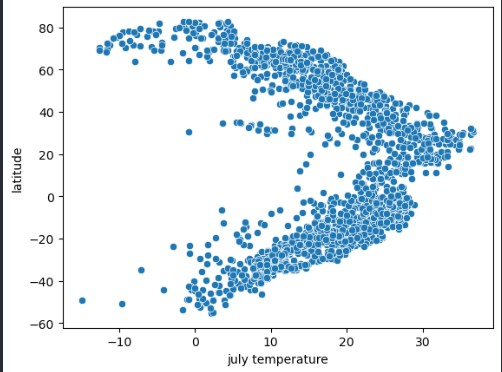
\includegraphics[width=10cm]{homework/homework_1/scatter_1.jpg}
    \item 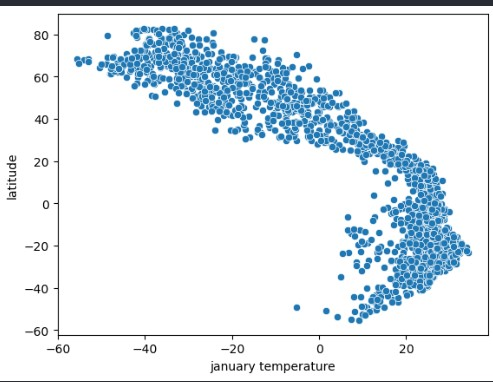
\includegraphics[width=10cm]{homework/homework_1/scatter_2.jpg}
    \item i found that $\rho$ for latitude and January was -0.880824383893164. that suggest a fairly strong negative linear relationship between longitude and the average temperature in January which does not seem to be supported by the graph 
    \item and for July and latitude it was  -0.09081110315246894. this suggests a week negative relationship, between average temperature and latitude in July, but it seems that there is a strong linear relationship present in the scatter plot if we segment the data based on if one is above or bellow 0 latitude. 
    
    \end{itemize}
	\item Compute the correlation between latitude and temperature in July for the locations in the southern hemisphere (latitude $< 0$). Plot scatterplots and the linear MMSE estimator and corresponding residuals.

 \begin{itemize}
     \item  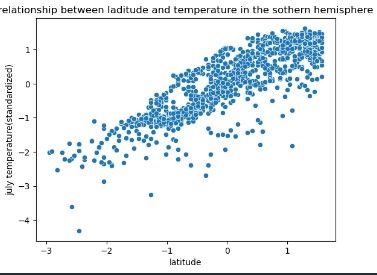
\includegraphics[width=10cm]{homework/homework_1/north_1.jpg}
 \item  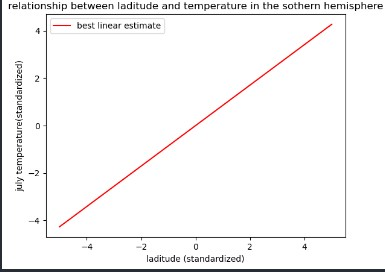
\includegraphics[width=10cm]{homework/homework_1/north_2.jpg}
 \item  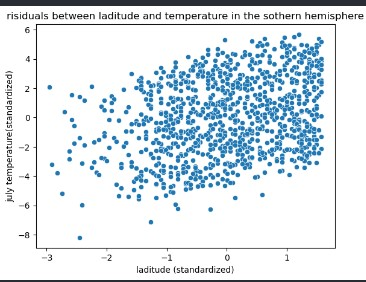
\includegraphics[width=10cm]{homework/homework_1/north_3.jpg}
 \end{itemize}
	\item Repeat the experiment for locations in the northern hemisphere (latitude $> 0$) in January. Explain your findings.

  \begin{itemize}
     \item  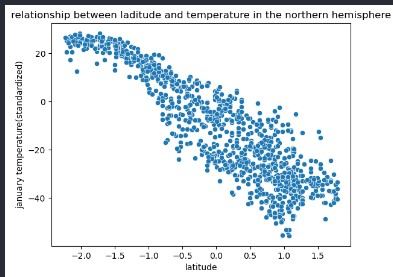
\includegraphics[width=10cm]{homework/homework_1/south_1.jpg}
 \item  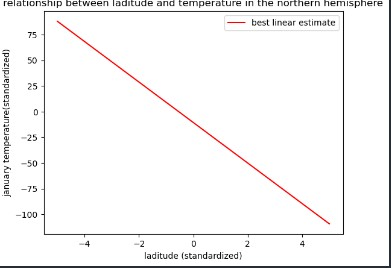
\includegraphics[width=10cm]{homework/homework_1/south_22.jpg}
 \item  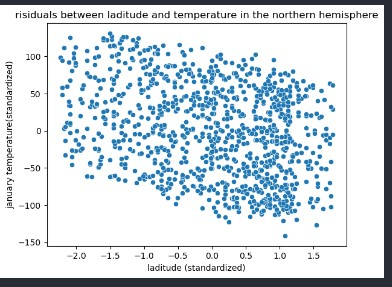
\includegraphics[width=10cm]{homework/homework_1/south_33.jpg}
 \item in the southern hemisphere in July there is a strong positive linear connection between average temperature and latitude as evidence by the charts in part b , further the relationship has $\rho=0.85395731$
 \item conversely in the northern hemisphere in January there is a strong negative linear correlation between average temperature and latitude as evidenced by the charts in part c, further the relationship has $\rho=-0.90442828$
 \end{itemize}
\end{enumerate}


\end{enumerate}
\end{document}
